% !TEX root = ../master-thesis.tex


\begin{figure}
    \centering
    \addletter{125}{a}
    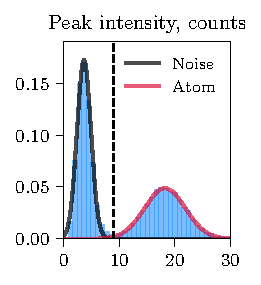
\includegraphics{fig-py/imaging-hist.pdf}
    \hfill
    \addletter{125}{b}
    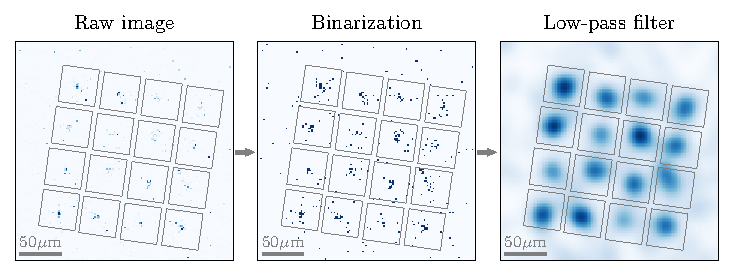
\includegraphics{fig-py/imaging-base.pdf}
    \caption[Single-atom identification and image processing]{
        \textbf{Single-atom identification and image processing.}
        a) Histogram of peak intensities extracted from binarized and low-pass filtered images shows a bimodal distribution: the first peak corresponds to camera noise (black), the second corresponds to single atoms (red). The dashed line indicates the threshold used for atom identification.
        b) Image processing pipeline: Raw fluorescence image (left), binarization by intensity thresholding (center), and application of a low-pass filter (right) to reveal spatially localized atomic signals. 
        % \red{Для (a) можно добавить fit, показав что иногда случаются и два атома.}
    }
    \label{fig:imaging}
\end{figure}

% \textbf{Camera and detection regime.}  
The imaging system uses a Nüvü HNü512 EMCCD camera, chosen for its high sensitivity and low noise in the few-photon regime. At $\lambda = 671$~nm, the sensor achieves a quantum efficiency (QE) of approximately 94\%~\cite{kruip_design_2024}. The camera is operated in photon counting mode with EM gain up to 5000, enabling single-atom detection from just tens of detected photons. During a typical imaging sequence, each atom emits around 300 photons, of which approximately 30 are detected on the camera after collection and transmission losses.

% \textbf{Binarization and filtering pipeline.}  
To mitigate the excess noise factor (ENF) inherent in EM amplification and to suppress clock-induced charges (CICs), we apply a binarization scheme. A fixed threshold (typically $5\sigma_\text{read}$ above the baseline noise) is used to convert raw images into binary maps, where each pixel is marked as "bright" if it exceeds the threshold and "dark" otherwise. This removes ambiguity due to the stochastic gain distribution and allows images to be treated as photon arrival maps.  

To reduce high-frequency noise while preserving localized atomic signals, we apply a Gaussian low-pass filter with a tunable width (typically $\sigma = 7$ px, close to the diffusion scale). This smooths the binarized images and helps identify spatially coherent clusters corresponding to single atoms. 
% \red{Optionally, a denoising step based on a circular neighbor-count kernel can be applied after binarization; see Appendix for implementation details.}

% \textbf{Atom identification from local maxima.}  
We locate candidate atom positions by searching for local maxima in the filtered images. Since the imaging beam is symmetric and atoms are spatially separated (due to the tweezer geometry), each atom forms a compact signal peak. To distinguish real atoms from CIC-induced noise clusters, we construct a histogram of peak amplitudes and apply a classification threshold based on the bimodal structure (see Fig.~\ref{fig:imaging}). This provides a robust method for single-atom detection within each image.

% \textbf{Use of ROI and regular array geometry.}  
During this work, all experiments were performed with a regular tweezer array. This allows us to restrict image analysis to known regions of interest (ROIs) around each expected atom location. This prior knowledge significantly simplifies the classification problem: we identify the atom at a given site as present or absent based on the presence of a peak in the corresponding ROI. This enables more reliable classification than in fully general imaging tasks as in \cite{bergschneider_spin-resolved_2018}.

% \textbf{Implementation and contribution.}  
The entire image analysis pipeline (bias correction, binarization, optional denoising, filtering, and classification) was implemented by the author in Python. The resulting code is vectorized and supports batch processing of image sequences. While the core concepts draw from existing methods developed in~\cite{bergschneider_spin-resolved_2018}, the current implementation is adapted to the geometry and noise characteristics of our setup. 
% Notably, the simplification due to known array geometry enables efficient and accurate analysis suitable for high-throughput acquisition.
